\subsection{Сферическая тригонометрия}
\label{sec:spher-trig}
\begin{wrapfigure}[10]{r}{.3\tw}
    \centering
    \vspace{-1pc}
    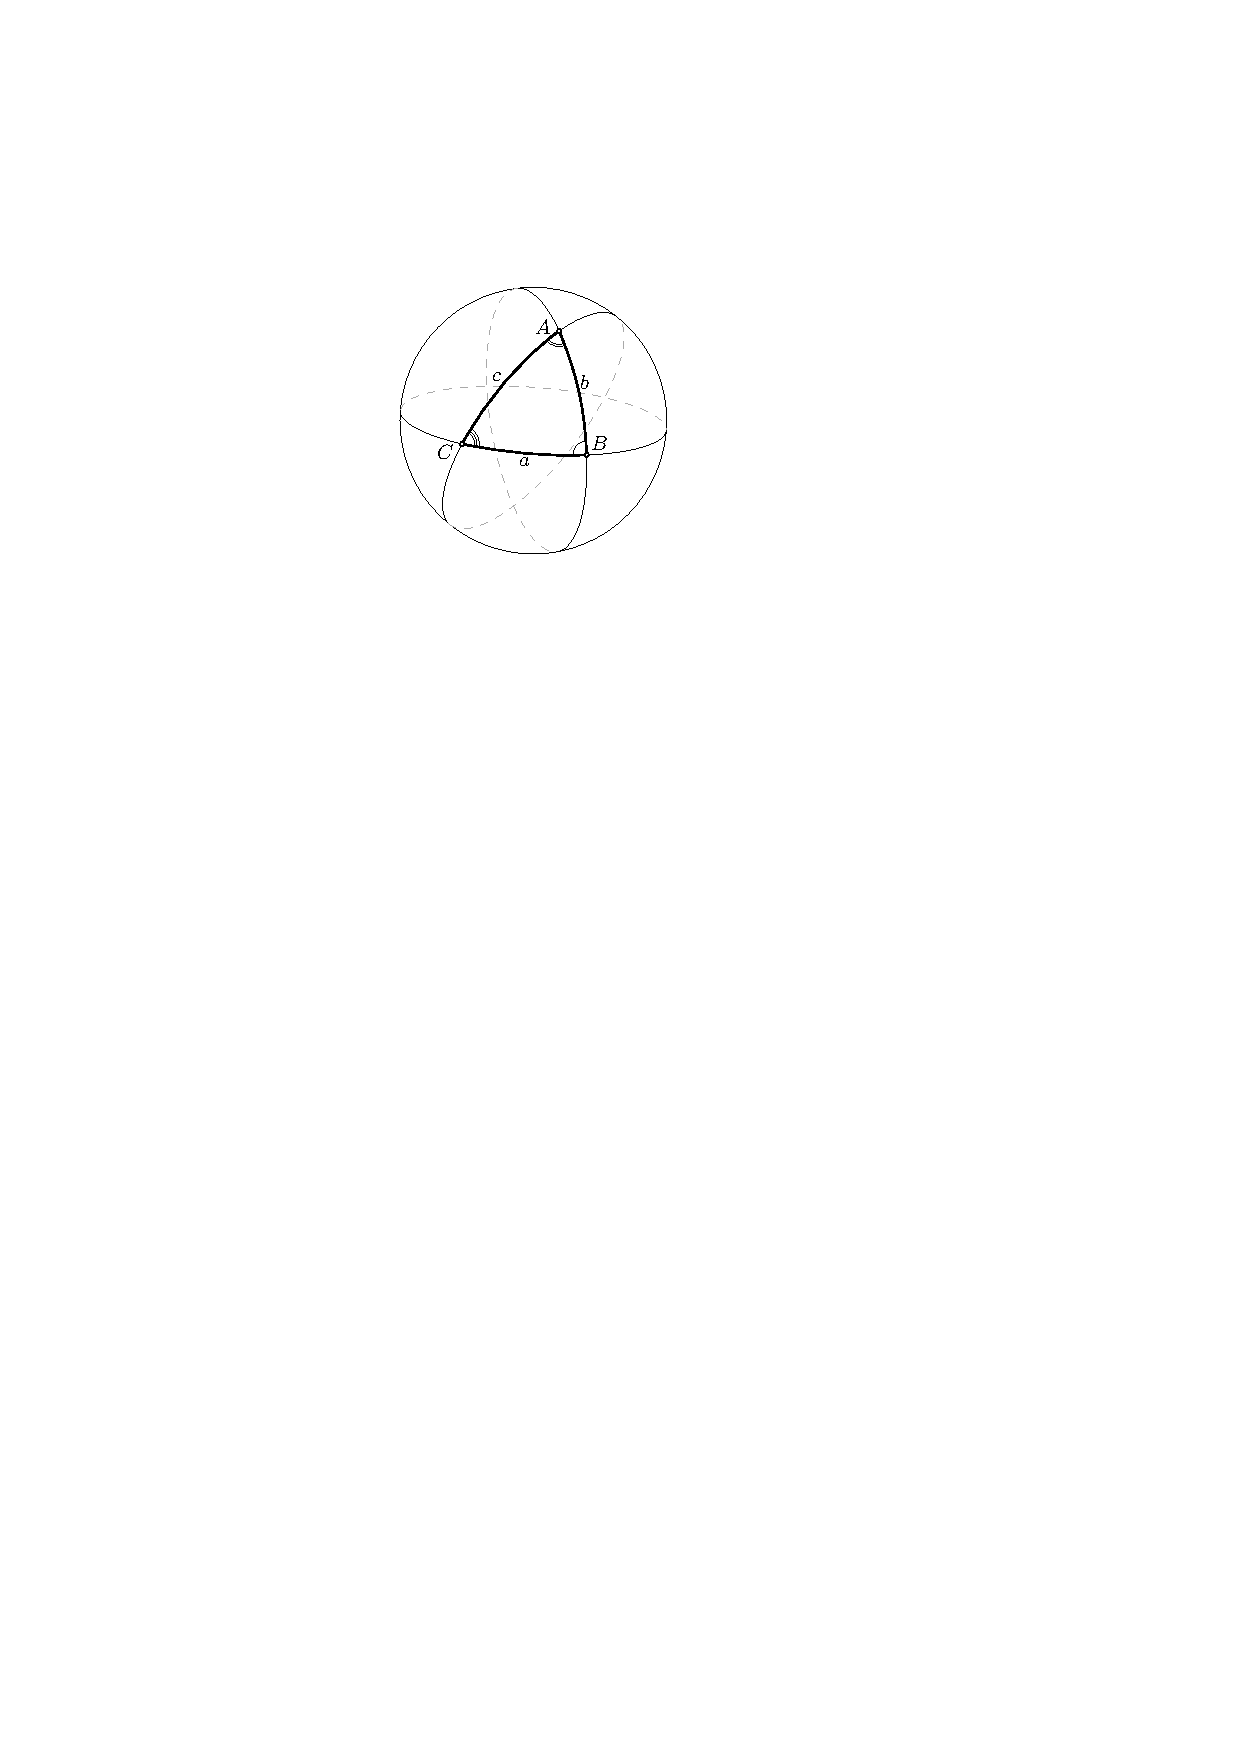
\includegraphics[width=0.3\textwidth]{spher-trigonom}
    \caption{Сферический треугольник}
\end{wrapfigure}
Для решения некоторых задач астрономии, связанных с видимыми положениями небесных тел, требуются знания о сферической тригонометрии. \imp{Сферический треугольник}~--- фигура на поверхности сферы, состоящая из трёх точек и трёх дуг больших кругов, соединяющих эти точки. Пусть $A$, $B$ и $C$~--- углы сферического треугольника, а $a$, $b$ и $c$~--- его стороны.

Сферические треугольники обладают следующими свойствами:
\begin{enumerate}
    \item Два сферических треугольника равны, если они подобны.
    \item Каждая сторона меньше суммы двух других сторон и больше их разности.
    \item Сумма всех сторон $a+b+c$ всегда меньше $2\pi$.
    \item Сумма углов сферического треугольника $\pi < A + B + C < 3\pi$.
    \item Разность суммы двух углов и третьего угла меньше $\pi$
\end{enumerate}

Площадь сферического треугольника определяется по формуле:
\begin{equation}
    S = R^2( A + B + C - \pi),
\end{equation}
где $A + B + C - \pi$~--- \imp{сферический избыток}.

Рассмотрим сферический треугольник $ABC$, радиус векторы вершин соответственно $\vec{a}$, $\vec{b}$ и $\vec{c}$.Причем из определения сферы $|\vec{a}| = |\vec{b}| = |\vec{c}| = r$. Пусть против вершин $A$, $B$ и $C$ лежат стороны с угловой мерой $a$, $b$ и $c$ соответсвенно. Повернем сферические координаты и нормируем так, чтобы $\vec{a} = (0, 0, 1)$, $\vec{b} = (\sin c, 0, \cos c)$, тогда $ \vec{c} = (\sin b \cos A, \sin b \sin A, \cos b)$.

Теперь запишем выражение для $\scalar{b}{c}$:
\begin{equation}
    \scalar{b}{c} = \cos a = \sin c \sin b \cos A + \cos c \cos b.
    \label{eq:spher-astro-cos-1}
\end{equation}
Аналогично,
\begin{gather}
    \scalar{a}{c} = \cos b = \sin a \sin c \cos B +  \cos a \cos c,\\
    \scalar{a}{b} = \cos c = \sin a \sin b \cos C + \cos a \cos b.
    \label{eq:spher-astro-cos-1-1}
\end{gather}
Выразим отсюда $\cos A$:
\begin{equation}
    \cos A = \frac{\cos a - \cos c \cos b}{\sin c \sin b}.
    \label{eq:spher-astro-cos-2}
\end{equation}
Формулы \eqref{eq:spher-astro-cos-1}\,--\,\eqref{eq:spher-astro-cos-2} называются \term{сферической теоремой косинусов} \imp{для стороны} \eqref{eq:spher-astro-cos-1}\,--\,\eqref{eq:spher-astro-cos-1-1} и, соответственно \imp{для угла} \eqref{eq:spher-astro-cos-2}.

Из основного тригонометрического тождества имеем:
\begin{multline*}
    \sin^2 A = 1 - \cos^2 A = 1 - \left[ \frac{\cos a - \cos c \cos b}{\sin c \sin b} \right]^2 = \\
    = \frac{\sin^2 c \sin^2 b - \cos^2 a + 2\cos a \cos c \cos b - \cos^2 c \cos^2 b}{\sin^2 c \sin^2 b}=\\
    = \frac{(1 - \cos^2 c)(1 -  \cos^2 b) - \cos^2 a + 2\cos a \cos c \cos b - \cos^2 c \cos^2 b}{\sin^2 c \sin^2 b}=\\
    = \frac{1 - \cos^2 c - \cos^2 b + \cos^2 c \cos^2 b -\cos^2 a}{\sin^2 c \sin^2 b} + \\
    + \frac{2\cos a \cos c \cos b - \cos^2 c \cos^2 b}{\sin^2 c \sin^2 b} = \\
    = \frac{1 - \cos^2 c - \cos^2 b - \cos^2 a + 2\cos a \cos c \cos b}{\sin^2 c \sin^2 b}.
\end{multline*}
Извлекая квадратный корень из левой и правой части и деля их на $\sin a$ имеем
\begin{equation*}
    \frac{\sin{A}}{\sin a} = \frac{\sqrt{1 - \cos^2 c - \cos^2 b - \cos^2 a + 2\cos a \cos c \cos b}}{\sin a \sin b \sin c}.
\end{equation*}
Заметим, что правая часть равенства циклична по переменным $a$, $b$ и $c$, следовательно, \term{сферическая теорема синусов} имеет вид
\begin{equation}
    \frac{\sin A}{\sin a} = \frac{\sin B}{\sin b} = \frac{\sin C}{\sin c}.
    \label{eq:sphere-th-sinus}
\end{equation}

Далее получим \term{формулу пяти элементов}. Для этого запишем теорему косинусов в выразим в ней один из косинусов, применяя ее же:
\begin{gather}
    \cos a = \sin c \sin b \cos A + \cos c \cos b,\nonumber\\
    \cos a = \sin c \sin b \cos A + \left( \sin a \sin b \cos C + \cos a \cos b \right)\cos b,\nonumber\\
    \cos a - \cos a \cos^2 b = \sin c \sin b \cos A + \sin a \sin b \cos b \cos C,\nonumber\\
    \cos a \sin^2 b = \sin c \sin b \cos A + \sin a \sin b \cos b \cos C,\nonumber\\
    \cos a \sin b = \sin a \cos b \cos C + \sin c \cos A.
    \label{eq:formula-5-elem}
\end{gather}


\begin{wrapfigure}[14]{r}{0.5\tw}
    \centering
    \vspace{-1pc}
    \tikzsetnextfilename{navigation-triangle}
    \tdplotsetmaincoords{70}{170}
    \begin{tikzpicture}[tdplot_main_coords]
        \footnotesize
        
        \def\r{2.5}
        \def\f{55}
        \def\d{20}
        \def\l{100}
        \def\t{60}


        % Draw spherical grid
        \draw[tdplot_screen_coords,thin,black!30] (0,0,0) circle (\r);
        \foreach \a in {-60,-30,...,60}{
            \tdplotCsDrawLatCircle[thin,black!20]{\r}{\a}
        }
        \foreach \a in {0,30,...,150}{
            \tdplotCsDrawLonCircle[thin,black!20]{\r}{\a}
        }
    
        
        % Delta coord of the intersection horizon and circle of equal right ascention
        \pgfmathsetmacro{\deltaMin}{atan(-cos(\t)/tan(\f))}
        
        % Angle between horizon and circle of equal right ascention
        \pgfmathsetmacro{\rotateAngle}{asin(cos(\t) * cos(\f) / sin(\deltaMin))}
        
        % 90 - Azimuth coord of the intersection horizon and circle of equal right ascention
        \pgfmathsetmacro{\AA}{acos(sin(\t) * cos(\deltaMin))}
        
        
        \pgfmathsetmacro\z{acos(sin(\f)*sin(\d) + cos(\f)*cos(\d)*cos(\t)}
        \pgfmathsetmacro\a{asin(cos(\d) * sin(\t) / sin(\z))}
        
    
        % Draw main azimuthal directions
        \draw [gray] (0,\r,0) -- (0,-\r,0);
        \draw [gray] (\r,0,0) -- (-\r,0,0);
        
        
        % Mark  and label angle A and 180 - A near Z
        \draw [double, fill=none, line cap=butt]({0.3*cos(180-\a - 3)},{0.3 * sin(180-\a -3)},\r) arc (180-\a-3:5:0.3);
        \tdplotCsLabelPoint{\r}{0}{0}{\adjustbox{right=10pt}{\scriptsize$180 \! - \!\!A$}}{below=3pt}
        
        
        % Mark and label angle t near P
        \def\angleRadius{0.4}
        \tdplotsetrotatedcoords{0}{-\f}{0};
        \draw [tdplot_rotated_coords, canvas is yz plane at x = \r]({\angleRadius * cos(80)},{\angleRadius * sin(80)}) arc (80:{90 - \t - 5}:\angleRadius);
        \tdplotCsLabelPoint{\r}{0}{90 - \f}{\adjustbox{raise=6pt}{$t$}}{right=9pt}
        
        
         % Mark right angles
        \tdplotsetrotatedcoords{0}{0}{180 - \a};
        \draw [tdplot_rotated_coords](\r,0.2,0.2) coordinate (c) (\r,0.2,0) coordinate (a1) -- (c) (\r,0,0.2) coordinate (a2) -- (c) pic [angle radius=0.2cm] {right angle=a1--c--a2};
        
        \tdplotsetrotatedcoords{0}{90 - \f}{180 - \t};
        \draw [tdplot_rotated_coords](\r,0.2,0.2) coordinate (c) (\r,0.2,0) coordinate (a1) -- (c) (\r,0,0.2) coordinate (a2) -- (c) pic [angle radius=0.2cm] {right angle=a1--c--a2};
        
        
        % Draw triangle
        \tdplotsetrotatedcoords{-90}{-90}{0};
        \draw[tdplot_rotated_coords, thick] (\r,0,0) arc (0:{90 -  \f}:\r);
        \tdplotsetrotatedcoords{\AA}{\rotateAngle}{\deltaMin};
        \draw[tdplot_rotated_coords, thick] (\r,0,0) arc (0:{90 - \d}:\r);
        \tdplotsetrotatedcoords{90 - \a}{-90}{0};
        \draw[tdplot_rotated_coords, thick] (\r,0,0) arc (0:\z:\r);
        
        
        %%%% Draw great circles
        % Celestial equator
        \tdplotCsDrawGreatCircle[semithick, tdplotCsFill/.style={opacity=0.0}]{\r}{0}{90 - \f}
        % Circle of equal azimuths
        \tdplotCsDrawGreatCircle[tdplotCsFill/.style={opacity=0.0}]{\r}{90 -\a}{90}
        % Celestial meridial
        \tdplotCsDrawGreatCircle[tdplotCsFill/.style={opacity=0.0}]{\r}{90}{90}
        % Circle of equal right ascension
        \tdplotCsDrawGreatCircle[tdplotCsFill/.style={opacity=0.0}]{\r}{180 + \AA}{180 - \rotateAngle}
        % Horizon
        \tdplotCsDrawLatCircle[semithick,tdplotCsFill/.style={opacity=0.00}]{\r}{0}

        
        % Draw and label points
        \tdplotCsDrawPoint{\r}{0}{90}
        \tdplotCsLabelPoint{\r}{0}{90}{$N$}{left}
        
        \tdplotCsDrawPoint{\r}{90}{90}
        \tdplotCsLabelPoint{\r}{90}{90}{$W$}{below right=-2pt}
        
        \tdplotCsDrawPoint{\r}{180}{90}
        \tdplotCsLabelPoint{\r}{180}{90}{$S$}{right}
        
        \tdplotCsDrawPoint{\r}{270}{90}
        \tdplotCsLabelPoint{\r}{270}{90}{$E$}{above}
        
        \tdplotCsDrawPoint{\r}{0}{0}
        \tdplotCsLabelPoint{\r}{0}{0}{$Z$}{above}
        
        \tdplotCsDrawPoint{\r}{0}{90 - \f}
        \tdplotCsLabelPoint{\r}{0}{90 - \f}{$P$}{above}
        
        \tdplotCsLabelPoint{\r}{90 + \a / 2}{88}{$A$}{above right = 3pt}
        
        
        % Label arcs
        \tdplotCsLabelPoint{\r}{0}{45 - \f / 2}{\adjustbox{right=12pt}{$90 - \varphi$}}{above}
        \tdplotCsLabelPoint{\r}{135 - \a / 2}{\z / 2}{$z$}{right=5pt}
        \tdplotCsLabelPoint{\r}{90 - \a / 2}{(90 - \f + \z) / 2}{\adjustbox{left=15pt}{$90 - \delta$}}{below=-13pt}
        \tdplotCsLabelPoint{\r}{180 - \t / 1.5}{45 + \f / 3}{$t$}{right}
        \tdplotCsLabelPoint{\r}{180 - \a + 6}{\z + (90 - \z) / 5}{$\delta$}{right}
        \tdplotCsLabelPoint{\r}{180 - \a}{\z + (90 - \z) / 2}{$h$}{left=-1pt}
        
        
        % Draw intersection oof celestial equator and celestial meridian
        \tdplotCsDrawPoint{\r}{180}{\f}
        
        % Draw star's projection on horizon
        \tdplotCsDrawPoint{\r}{180-\a}{90}
        
        % Draw star's projection on celestial equator
        \pgfmathsetmacro{\zz}{acos(cos(\f)*cos(\t)}
        \pgfmathsetmacro{\aa}{180 - asin(sin(\t) / sin(\zz))}
        \tdplotCsDrawPoint{\r}{\aa}{\zz}
        
        % Draw star
        \draw ({\r * cos(180 - \a) * sin(\z)}, {\r * sin(180 - \a) * sin(\z)}, {\r * cos(\z)}) node[star, star points=5, star point ratio=2.25, fill=black, scale=0.35] {};
        
        % Draw the center of sphere
        \tdplotCsDrawPoint{0}{0}{0}
    \end{tikzpicture}

    \caption{Параллактический треугольник}
    \label{pic:paralactic-triangle}    
\end{wrapfigure}

\term{Параллактический треугольник}~--- треугольник на небесной сфере, образованный пересечением небесного меридиана, вертикального круга и часового круга светила. \imp{Вертикальный круг}~--- большой круг небесной сферы, проходящий через надир, зенит и светило. \imp{Часовой круг}~--- большой круг небесной сферы, проходящий через полюса мира и наблюдаемое светило.

Применяя теоремы синусов и косинусов к параллактическому треугольнику, нетрудно получить следующие соотношения:
\begin{gather}
    \cos z=\sin\varphi\sin\delta+\cos\varphi\cos\delta\cos t\\
    \sin z\sin A=\cos\delta\sin t\\
    \sin z\cos A=-\cos\varphi\sin\delta+\sin\varphi\cos\delta\cos t
\end{gather}

\begin{wrapfigure}[11]{r}{0.42\tw}
    \centering
    \vspace{-1.5pc}
    \tikzsetnextfilename{grand-circle-eq}
    \tdplotsetmaincoords{70}{155}
    \begin{tikzpicture}[tdplot_main_coords]
        \footnotesize

        \def\r{2}
        \def\i{25}
        \def\lo{70}
        \def\l{100}
        \def\f{atan(sin(\l - \lo) * tan(\i))}

        \def\x{asin(sin(\f) / sin(\i))}
        \def\q{atan(sin(\x) * tan(\i))}
        \def\y{asin(sin(\q) / sin(\i))}
        \def\w{asin(sin(\x) / sin(\y))}


        \draw[tdplot_screen_coords,thin,black!30] (0,0,0) circle (\r);
        \foreach \a in {-60,-30,...,60}{
            \tdplotCsDrawLatCircle[thin,black!30]{\r}{\a}
        }
        \foreach \a in {0,30,...,150}{
            \tdplotCsDrawLonCircle[thin,black!30]{\r}{\a}
        }

        \tdplotCsDrawLatCircle[thick,tdplotCsFill/.style={opacity=0.00}]{\r}{0}

        \tdplotCsDrawGreatCircle[thick,tdplotCsFill/.style={opacity=0.0}]{\r}{\lo-90}{\i}

        \tdplotsetrotatedcoords{\y - 90 + \lo}{180 - \w}{\q};
        \draw[tdplot_rotated_coords, line width=1pt] (0,\r,0) arc (90:180:\r);
        \draw[tdplot_rotated_coords, anchor=north] (0,\r,0) node {\adjustbox{right=4mm,raise=-1mm}{$G$}};

        \tdplotsetrotatedcoords{\l - 90}{90}{\f};
        \draw[tdplot_rotated_coords, line width=1pt] (0,\r,0) arc (90:{180 -\f}:\r);

        \tdplotsetrotatedcoords{-180+\lo}{90}{90 - \i};
        \draw[tdplot_rotated_coords, line width=1pt] (0,\r,0) arc (90:{90+\i}:\r);

        \coordinate (P) at ({\r*cos(\lo - 90)*sin(\i)}, {\r*sin(\lo - 90)*sin(\i)},{\r*cos(\i)});
        \coordinate (P') at ({-\r*cos(\lo - 90)*sin(\i)}, {-\r*sin(\lo - 90)*sin(\i)},{-\r*cos(\i)});
        \draw[semithick, gray, dash dot, line cap=round] (P) -- (P');

        \def\x{asin(0.5/\r)}
        \tdplotsetrotatedcoords{-90+\lo+\x}{0}{0};
        \draw[tdplot_rotated_coords] (0,\r,0) arc (0:\i:5mm);

        \def\x{asin(0.2/\r)}
        \tdplotsetrotatedcoords{0}{-90 + \x}{-90 - \q};
        \draw[tdplot_rotated_coords] (0,\r,0) arc (200:315:2mm);

        \tdplotCsDrawPoint{\r}{\l}{90 - \f}

        \tdplotCsDrawPoint{\r}{\lo}{90}
        \tdplotCsLabelPoint{\r}{\lo}{90}{\adjustbox{left=4mm}{$(\lambda_0,0)$}}{anchor=north}

        \tdplotCsDrawPoint{\r}{\lo-90}{\i}
        \tdplotCsLabelPoint{\r}{\lo-90}{\i}{\adjustbox{left=5mm}{$P'$}}{anchor=south}

        \tdplotCsLabelPoint{\r}{0}{0}{}{label={[below]250:$\Delta \lambda$}}

        \tdplotCsDrawPoint{\r}{0}{0}
        \tdplotCsLabelPoint{\r}{0}{0}{$P$}{anchor=south}

        \tdplotCsLabelPoint{\r}{\lo-90}{\i/2}{$i$}{anchor=south}
        \tdplotCsLabelPoint{\r}{\l}{(90 - \f)/2 - 5}{$90^\circ - \varphi$}{anchor=west}
        \tdplotCsLabelPoint{\r}{\l - (\l - \lo + 90) /3 + 5}{(90 - \f + \i)/2 - 10}{$90^\circ$}{}

        \tdplotCsDrawPoint{\r}{0}{90}{}
        \tdplotCsLabelPoint{\r}{0}{90}{\adjustbox{left=2.5mm}{$(0,0)$}}{anchor= south}

        \tdplotCsDrawPoint{0}{0}{0}
    \end{tikzpicture}
    \caption{Произвольная точка $(\lambda, \varphi)$ на большом круге с полюсом $P'$}
    \label{pic:grand-circle}
\end{wrapfigure}
Напоследок, используя сферическую теорему косинусов, получим \term{уравнение большого круга}. Пусть на сфере заданы сферические координаты $(\lambda, \varphi)$, где $\lambda$~--- угол проекции вектора на плоскость $Oxy$ с осью $Ox$, см.~Раздел\;\ref{sec:coord-systems}, а $\varphi$~--- угол между вектором в плоскостью $Oxy$. Найдем уравнение большого круга с наклонением $i$, восходящий узел которого находится в точке $(\lambda_0, 0)$.

Для этого рассмотрим произвольную точку $G = (\lambda, \varphi)$ на этом большом круге и один из его полюсов $P' = (\lambda_0 - 90^\circ,\,90^\circ - i)$. По определению большого круга каждая его точка отстоит от полюса на $90^\circ$. Обозначим разность первых координат $P'$ и $G$~--- $\lambda - (\lambda_0 - 90^\circ)$, за $\Delta \lambda$ и запишем сферическую теорему косинусов для $\triangle PP'G$, где $P$~--- полюс заданной системы координат:
\begin{gather}
    \cos 90^\circ = \cos i \cos (90^\circ - \varphi) + \sin i \sin (90^\circ - \varphi) \cos \Delta \lambda,\nonumber \\
    0 = \cos i \sin \varphi - \sin i \cos \varphi \sin (\lambda - \lambda_0),\nonumber\\
    \frac{\tg \varphi}{\tg i} = \sin (\lambda - \lambda_0),
    \label{eq:great-circle-eq}
\end{gather}
полученное уравнение является \imp{уравнением большого круга}.
